
\section{Figures and Tables}


\noindent{\bf Figure 1.  Statistical errors of {\tt TESS3} and {\tt TESS 2.3} estimates.} Computer simulations of admixed populations using known individual ancestry proportions from two ancestral gene pools. A) RMSEs of $G$ estimates as a function of the level of ancestral population differentiation ($F_{\rm ST}$). B) RMSEs of $Q$ estimates as a function of the level of ancestral population differentiation ($F_{\rm ST}$).

\vspace{1cm}

\noindent{\bf Figure 2. Run-times for {\tt TESS3} and {\tt TESS 2.3}}. The number of ancestral population ranged between $K = 1$ and $6$. Run-times were expressed in unit of minutes.

\vspace{1cm}

\noindent{\bf Figure 3. Results of the {\it Arabidopsis thaliana} data analysis with {\tt TESS3}}. A) Geographic maps of ancestry coefficients using $K = 3$ ancestral populations. B) Manhattan plot of $\log_{10}(p$-values) for the plant chromosome 5. The horizontal line corresponds to an expected FDR value of $q = 10^{-30}$. 

\vspace{1cm}

\noindent{\bf Figure 4. Candidate SNPs from a genome scan of{\it A. thaliana} chromosome 5.} A) Histogram of adjusted $p$-values. B) Spatial distribution of allele frequency for two top-hit SNPs located in the {\it VSP1} and {\it WAV2} genes.

\vspace{1cm}


\noindent{\bf Table1. Power to reject neutrality of {\tt TESS3} outlier tests for two simulated data sets.}


\clearpage
\newpage




\begin{figure}[h!]\centering
\begin{minipage}{0.49\textwidth}
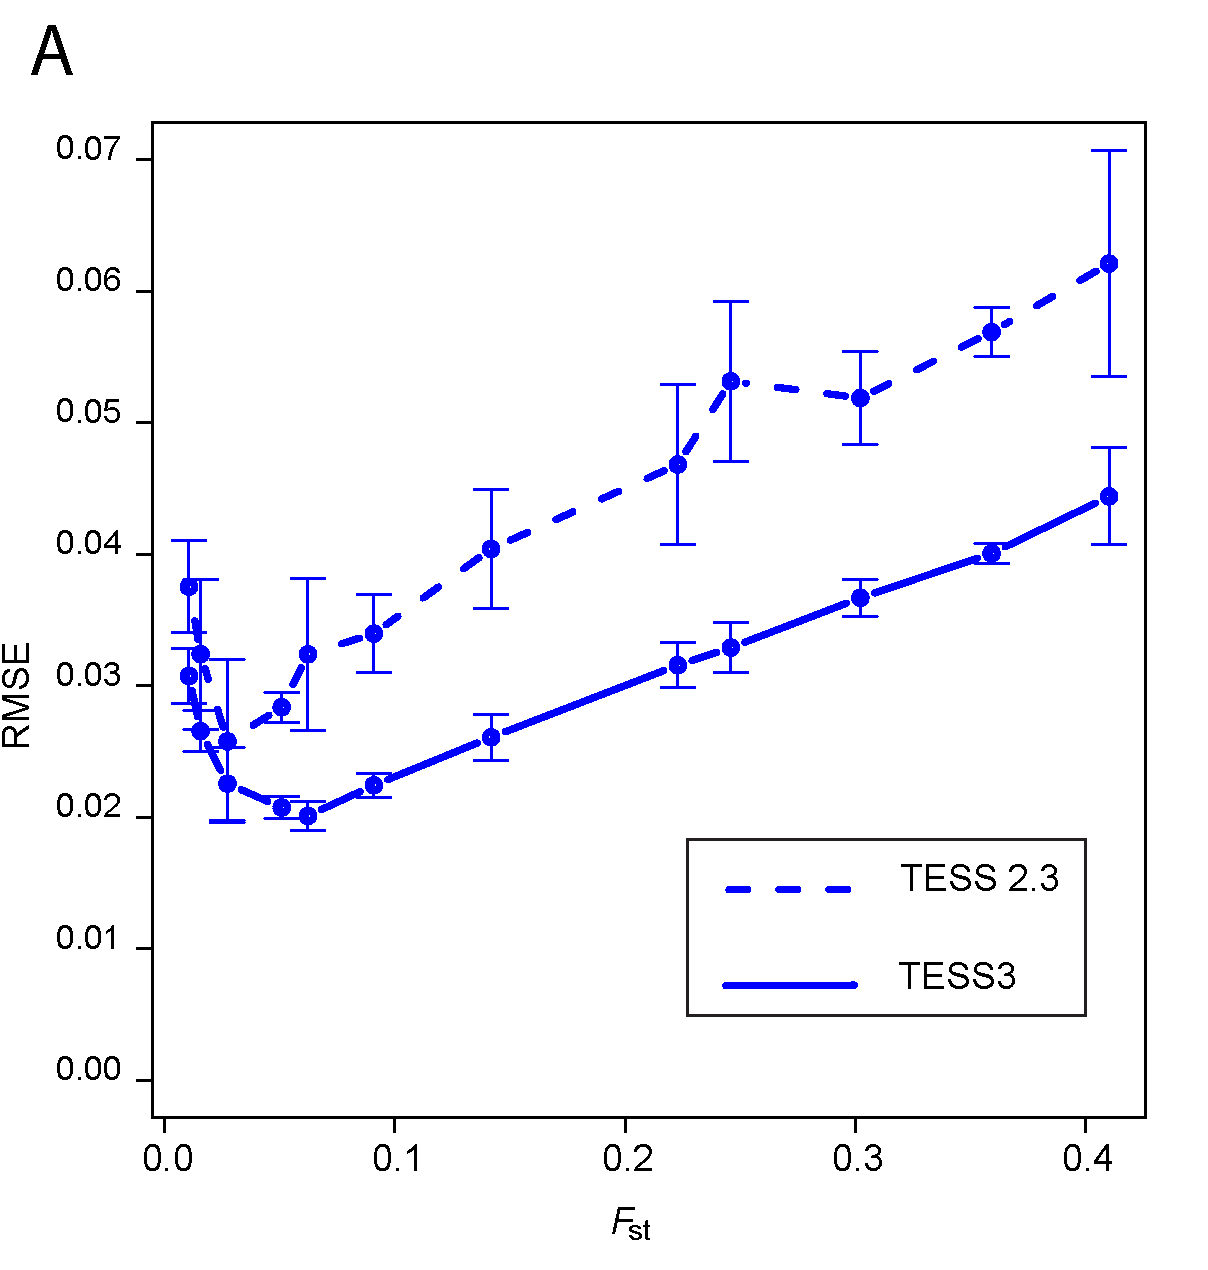
\includegraphics[width=\linewidth]{FinalGraphs/rmseG.pdf}
\end{minipage}
\begin {minipage}{0.49\textwidth}
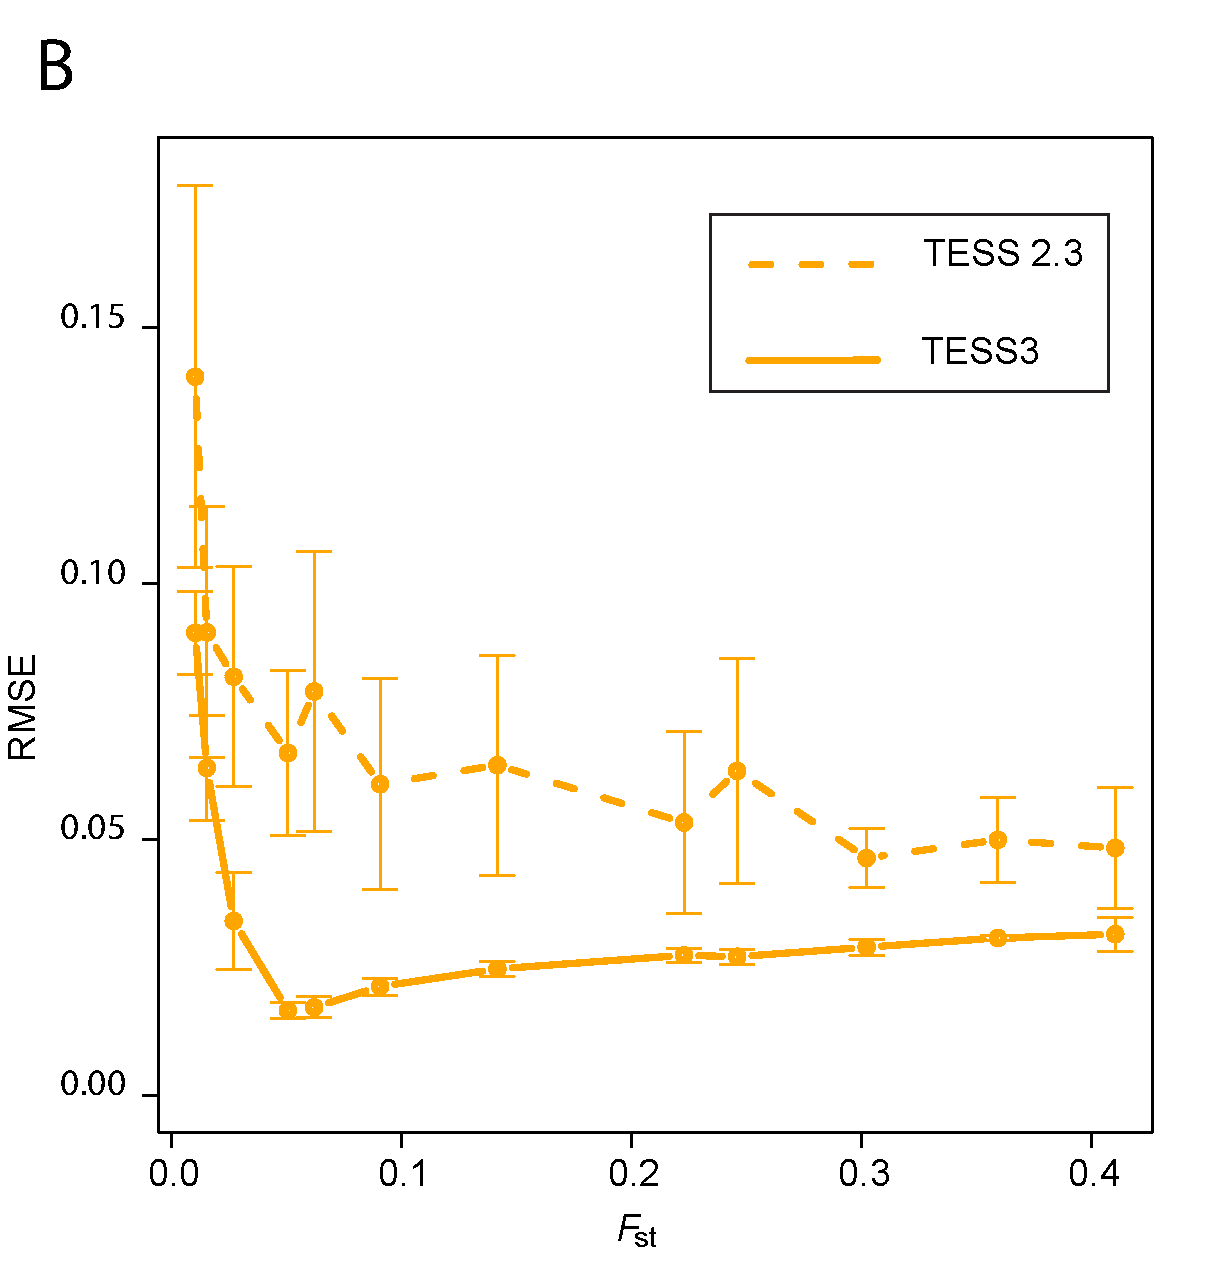
\includegraphics[width=\linewidth]{FinalGraphs/rmseQ.pdf}
\end{minipage}
\caption{Statistical errors of {\tt TESS3} and {\tt TESS 2.3} estimates. Computer simulations of admixed populations using known individual ancestry proportions from two ancestral gene pools. A) RMSEs of $G$ estimates as a function of the level of ancestral population differentiation ($F_{\rm ST}$). B) RMSEs of $Q$ estimates as a function of the level of ancestral population differentiation ($F_{\rm ST}$).}
\end{figure}    

\clearpage
\newpage



\begin{figure}[h!]
  \centering

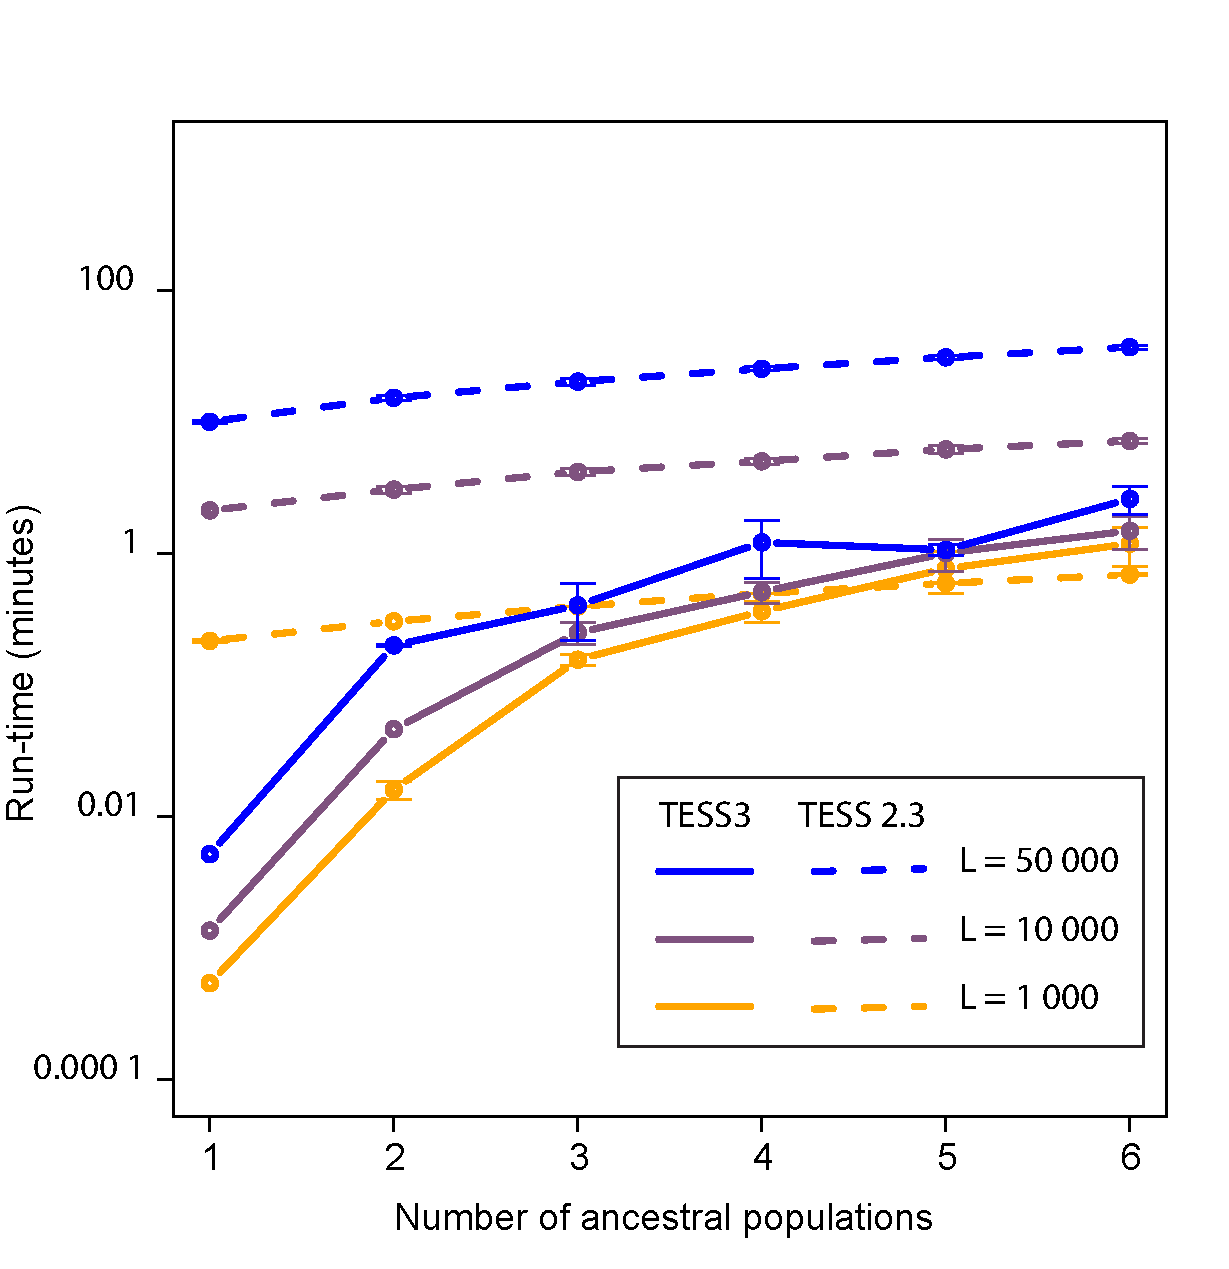
\includegraphics[width=\linewidth]{FinalGraphs/runtimes.pdf}
\caption{Run-times for {\tt TESS3} and {\tt TESS 2.3}.  The number of ancestral population ranged between $K = 1$ and $6$. Run-times were expressed in unit of minutes.}
\end{figure}

\clearpage
\newpage


\begin{figure}[h!]\centering
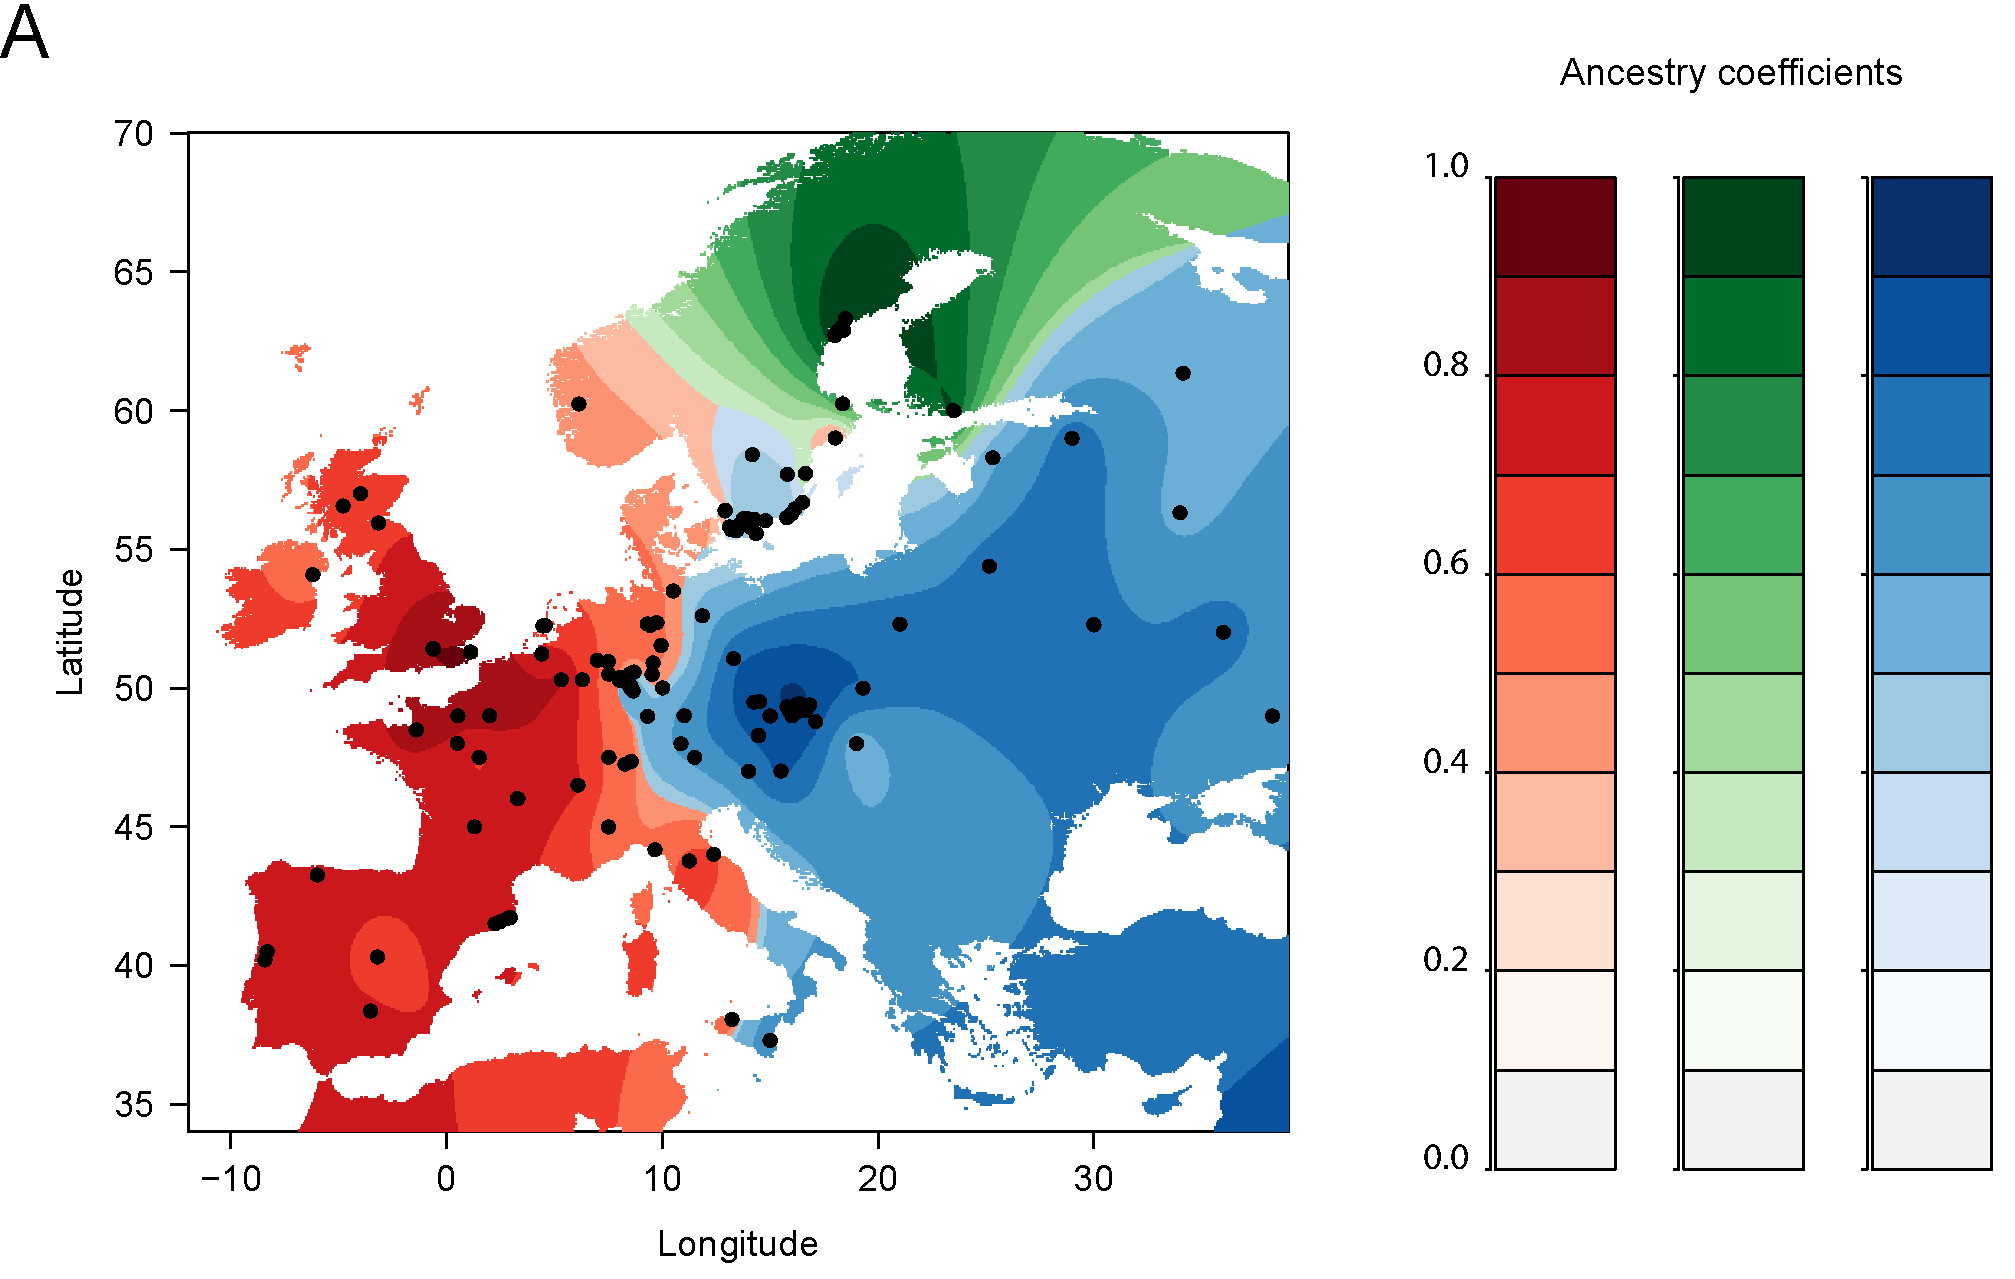
\includegraphics[width=\linewidth]{FinalGraphs/barsClusters.pdf}
\includegraphics[width=\linewidth]{FinalGraphs/manhattanPlot.pdf}
\caption{Results of the {\it Arabidopsis thaliana} data analysis with {\tt TESS3}. A) Geographic maps of ancestry coefficients using $K = 3$ ancestral populations. B) Manhattan plot of $\log_{10}(p$-values) for the plant chromosome 5. The horizontal line corresponds to an expected FDR value of $q = 10^{-30}$.}
\end{figure}    

\clearpage
\newpage 

\begin{figure}[h!]\centering
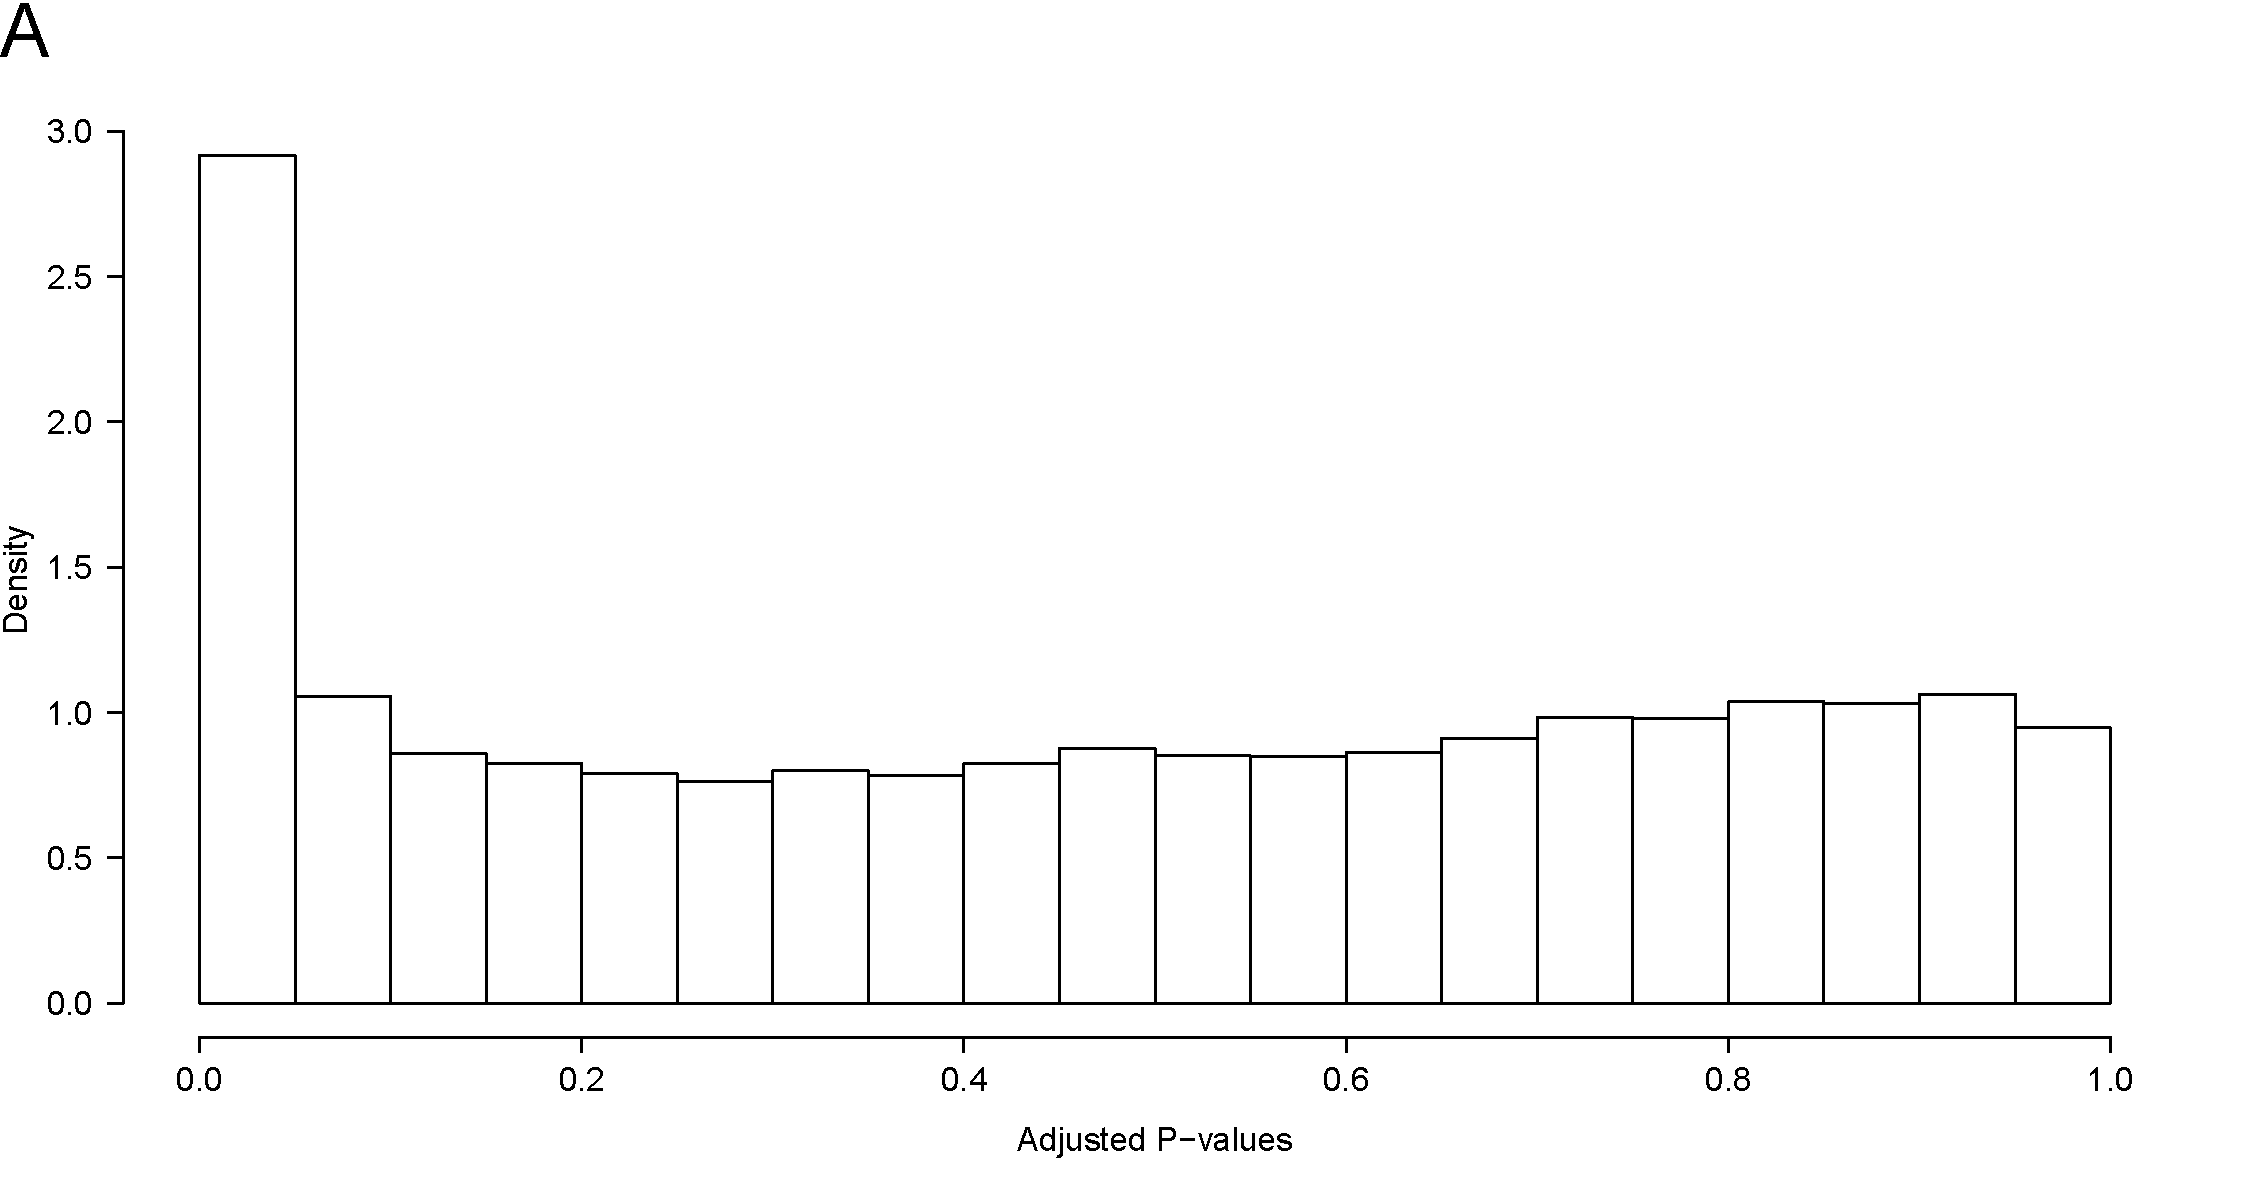
\includegraphics[width=\linewidth]{FinalGraphs/pValueHist.pdf}
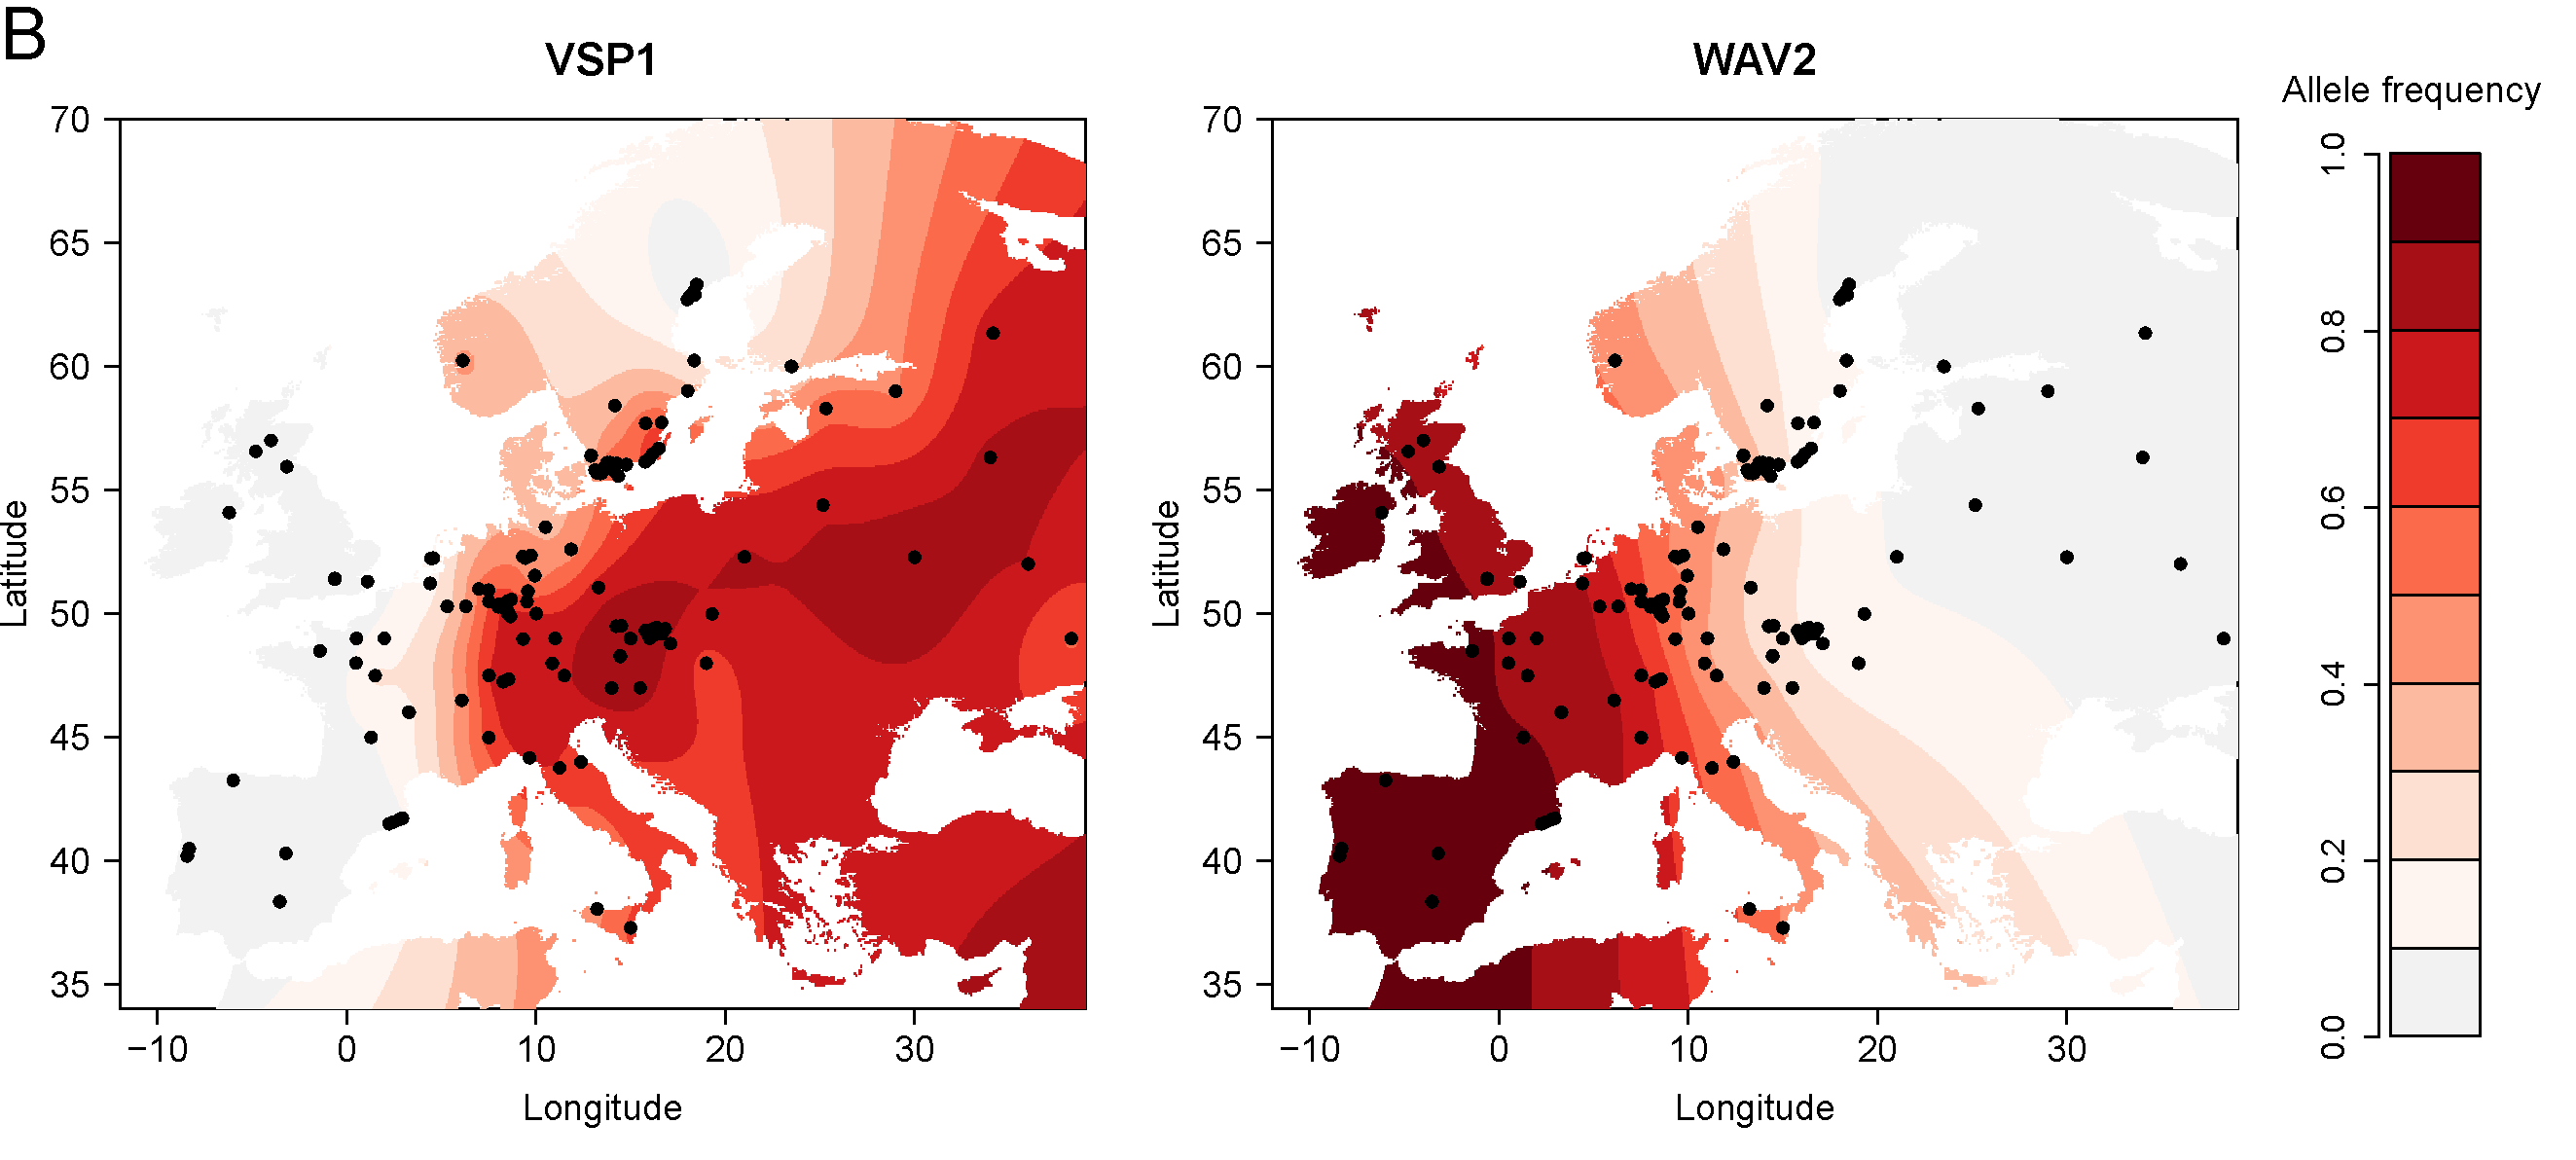
\includegraphics[width=\linewidth]{FinalGraphs/colorBar.pdf}
\caption{Candidate SNPs from a genome scan of the {\it A. thaliana} 5th chromosome. A) Histogram of adjusted $p$-values. B) Spatial distribution of allele frequency for two top-hit SNPs located in the {\it VSP1} and {\it WAV2} genes.}
\end{figure}    


\clearpage
\newpage 

\begin{table}
\noindent{\bf Table1. Power to reject neutrality of {\tt TESS3} outlier tests for two simulated data sets.}
\begin{center}
\begin{tabular}{lcccc}
 \hline
\textbf{FDR}  & \multicolumn{4}{c}{\textbf{Power}}  \\
 & After admixture & Before admixture & After admixture & Before admixture  \\
\hline
 0.05 & {\bf 0.61} & 0.63 & {\bf 0.20} & 0.26 \\
 0.10 & {\bf 0.63} & 0.66 & {\bf 0.23} & 0.29 \\
 0.15 & {\bf 0.64} & 0.67 & {\bf 0.25} & 0.32 \\
 0.20 & {\bf 0.65} & 0.69 & {\bf 0.26} & 0.33 \\
 \hline
\end{tabular}
\end{center}
\hspace{1cm}\noindent{\small Data set 1: $m_{\rm s} / m = 0.005$.  Data set 2: $m_{\rm s} / m = 0.05$.}
\end{table}

\clearpage	